%%%%%%%%%%%%%%%%%%%% book.tex %%%%%%%%%%%%%%%%%%%%%%%%%%%%%
%
% sample root file for the chapters of your "monograph"
%
% Use this file as a template for your own input.
%
%%%%%%%%%%%%%%%% Springer-Verlag %%%%%%%%%%%%%%%%%%%%%%%%%%


% RECOMMENDED %%%%%%%%%%%%%%%%%%%%%%%%%%%%%%%%%%%%%%%%%%%%%%%%%%%
\documentclass[pdftex,12pt, oneside, a4paper]{book}

% choose options for [] as required from the list
% in the Reference Guide, Sect. 2.2
%\usepackage[paperwidth=8.5in, paperheight=13in]{geometry}

\usepackage{makeidx}         % allows index generation
\usepackage{graphicx}        % standard LaTeX graphics tool
                             % when including figure files
\usepackage[bottom]{footmisc}% places footnotes at page bottom
\usepackage[english]{babel}
\usepackage{enumerate}
\usepackage{paralist}
\usepackage{float}
\usepackage{gensymb}  
\usepackage{listings}
\usepackage{color} 

% make quote in italic
\newenvironment{italicquotes}
  {\begin{quote}\itshape}
  {\end{quote}}
% etc.
% see the list of further useful packages
% in the Reference Guide, Sects. 2.3, 3.1-3.3

% definisi warna untuk kode program
\definecolor{codegreen}{rgb}{0, 0.6, 0}
\definecolor{codegray}{rgb}{0.5, 0.5, 0.5}
\definecolor{codepurple}{rgb}{0.58, 0, 0.82}
\definecolor{backcolor}{rgb}{0.95, 0.95, 0.92}

% list code custom style
\lstdefinestyle{mystyle} {
  backgroundcolor=\color{backcolor}, 
  commentstyle=\color{codegreen},
  keywordstyle=\color{magenta}, 
  numberstyle=\tiny\color{codegray},
  stringstyle=\color{codepurple},
  basicstyle=\footnotesize,
  breakatwhitespace=false, breaklines=true, captionpos=b, keepspaces=true,
  numbers=left, numbersep=5pt, showspaces=false, showstringspaces=false,
  showtabs=false, tabsize=2
}

% mystyle for listing set
\lstset{style=mystyle}

\newcommand{\HRule}{\rule{\linewidth}{0.5mm}}

\makeindex             % used for the subject index
                       % please use the style svind.ist with
                       % your makeindex program


%%%%%%%%%%%%%%%%%%%%%%%%%%%%%%%%%%%%%%%%%%%%%%%%%%%%%%%%%%%%%%%%%%%%%

\begin{document}

%\author{Priyanto Tamami}
%\title{BUKU PETUNJUK OPERASIONAL SISTEM INFORMASI GEOGRAFIS UNTUK PBB-P2 DENGAN MAPINFO VERSI 8.0}
%\date{22 Desember 2015}
%\maketitle

\begin{titlepage}

\begin{center}
{\large BUKU PETUNJUK IMPLEMENTASI QUANTUM GEOGRAPHICAL INFORMATION SYSTEM (QGIS) UNTUK DASAR PEMETAAN PBB-P2}

\HRule\\[1cm]

PERIODE PENILAIAN TAHUN 2016\\[1cm]


\includegraphics[width=0.5\textwidth]{./resources/logo}\\[1cm]

Oleh :\\
Priyanto Tamami, S.Kom.\\
NIP 19840409 201001 1 025\\
Dinas Pendapatan dan Pengelolaan Keuangan\\
Pemerintah Kabupaten Brebes\\[1cm]

\vfill

Tim Penilai\\
Jabatan Fungsional Pranata Komputer\\
Badan Pusat Statistik\\
Brebes, 26 Mei 2016
\end{center}

\end{titlepage}

\frontmatter%%%%%%%%%%%%%%%%%%%%%%%%%%%%%%%%%%%%%%%%%%%%%%%%%%%%%%

%\include{dedic}
%\include{pref}

\begin{center}
{\huge \bfseries Lembar Pengesahan}\\[0.4cm]

\begin{tabular}{l c p{10cm}}
  Nama Kegiatan & : & Membuat Petunjuk Operasional Sistem Komputer \\
  Judul & : & BUKU PETUNJUK IMPLEMENTASI QUANTUM GEOGRAPHICAL INFORMATION SYSTEM (QGIS) UNTUK DASAR PEMETAAN PBB-P2 \\
\end{tabular}\\[2cm]

\begin{tabular}{c c}
  Disetujui oleh : & Disusun Oleh \\
  Kepala Seksi Pendataan, Penetapan, dan Keberatan & Pranata Komputer \\
  Pada tanggal 27 Mei 2016 & Selesai tanggal : 26 Mei 2016 \\
  & \\
  & \\
  & \\
  Fetiana Dwiningrum, SIP, M.Si. & Priyanto Tamami, S.Kom \\
  NIP 19880223 200701 2 001 & NIP 19840409 201001 1 025
\end{tabular}

\end{center} 

\tableofcontents
\listoffigures

\mainmatter%%%%%%%%%%%%%%%%%%%%%%%%%%%%%%%%%%%%%%%%%%%%%%%%%%%%%%%


\chapter{KONSEP DASAR SISTEM INFORMASI GEOGRAFIS (SIG)}

\begin{enumerate}[A.]
\item{Definisi}

Sistem Informasi Geografis (Geographic Information System / GIS) yang selanjutnya disebut SIG merupakan sistem informasi berbasis komputer yang digunakan untuk mengolah dan menyimpan data atau informasi geografis.

Secara umum pengertian SIG adalah sebagai berikut :
\begin{italicquotes}
Suatu komponen yang terdiri dari \textbf{perangkat keras, perangkat lunak, sumber daya manusia, dan data} yang bekerja bersama secara efektif untuk memasukkan, menyimpan, memperbaiki, memperbaharui, mengelola, memanipulasi, mengintegrasikan, menganalisa, dan menampilkan data dalam suatu informasi berbasis geografis.
\end{italicquotes}

Dalam pembahasan selanjutnya, SIG akan selalu diasosiasikan dengan sistem yang berbasis komputer, walaupun pada dasarnya SIG dapat dikerjakan secara manual, SIG yang berbasis komputer akan sangat membantu ketika data geografis merupakan data yang besar (dalam jumlah dan ukuran) dan terdiri dari banyak tema yang saling berkaitan.

SIG mempunyai kemampuan untuk menghubungkan berbagai data pada suatu titik tertentu di bumi, menggabungkannya, menganalisa, dan akhirnya memetakan hasilnya.

\item{Komponen SIG}
\end{enumerate}

\chapter{DATA SIG (Format dan Sumber Data)}


\chapter{INSTALASI QGIS}

Cara instalasi aplikasi QGIS berbeda antara menggunakan sistem operasi Windows dan sistem operasi Linux.

\begin{enumerate}[A.]

\item Instalasi QGIS di lingkungan Sistem Operasi Windows

Untuk sistem operasi Windows, perangkat lunak QGIS dapat di unduh secara gratis di \textit{website} resmi QuantumGIS dengan alamat http://qgis.org/ melalui berbagai macam \textit{web browser} seperti Firefox, Chrome, Opera, atau Internet Explorer. Tahapannya adalah sebagai berikut :

\begin{enumerate}[1.]

\item Pada kolom halaman di atas jendela \textit{browser}, masukan teks berikut dan tekan Enter : http://qgis.org/, sehingga muncul jendela pada gambar \ref{fig:qgishomepage} :

\begin{figure}
  \centering
  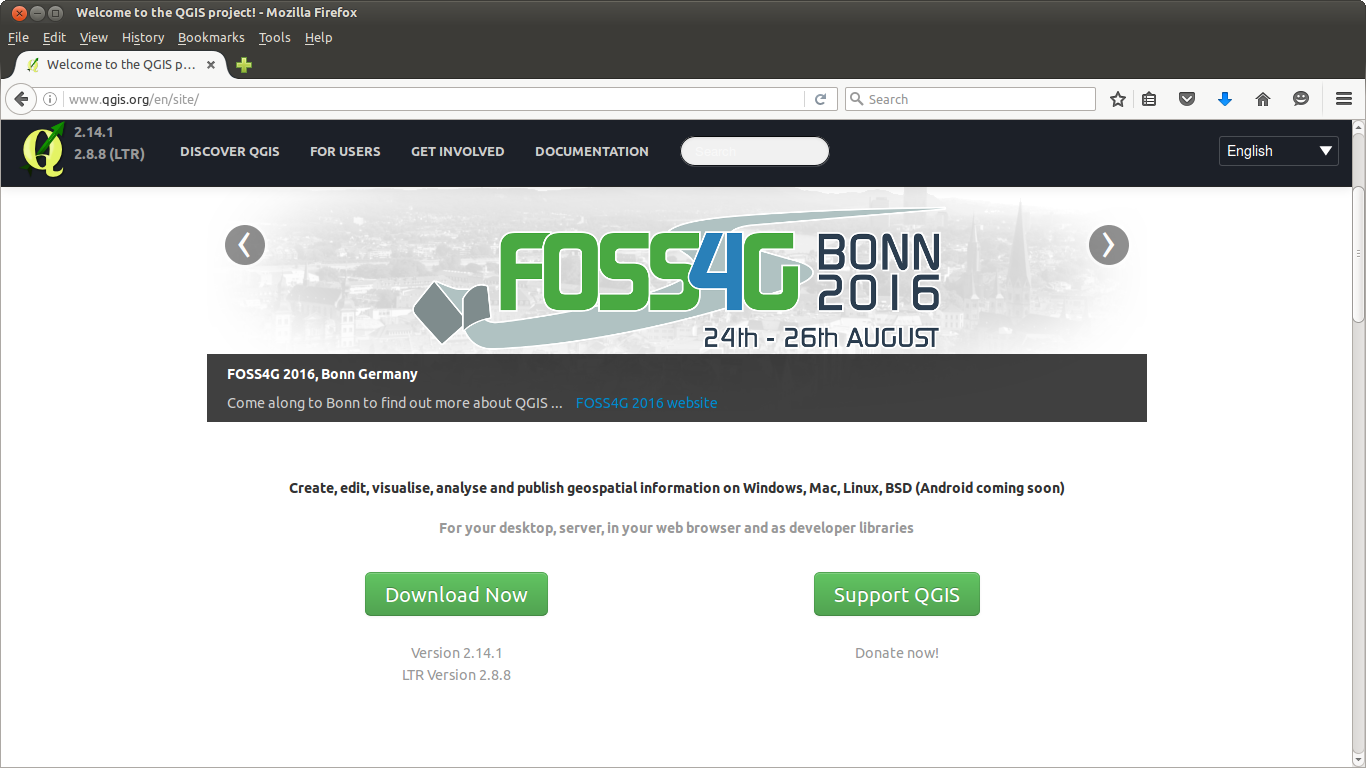
\includegraphics[width=1\textwidth]{./resources/001-homepage-qgis}
  \caption{Jendela \textit{website} QGIS}
  \label{fig:qgishomepage}
\end{figure}

\item Klik \verb|Download Now| pada halaman tersebut.

\item Pada jendela \textit{download} seperti ditampilkan dalam gambar \ref{fig:qgisversion} akan terdapat pilihan QGIS \textit{installer} berdasarkan sistem operasi perangkat yang anda gunakan. \textit{Expand} pilihan sistem operasi yang anda gunakan, lalu klik pada \textbf{Standalone Installer} (direkomendasikan untuk pengguna pemula).

\begin{figure}
  \centering
  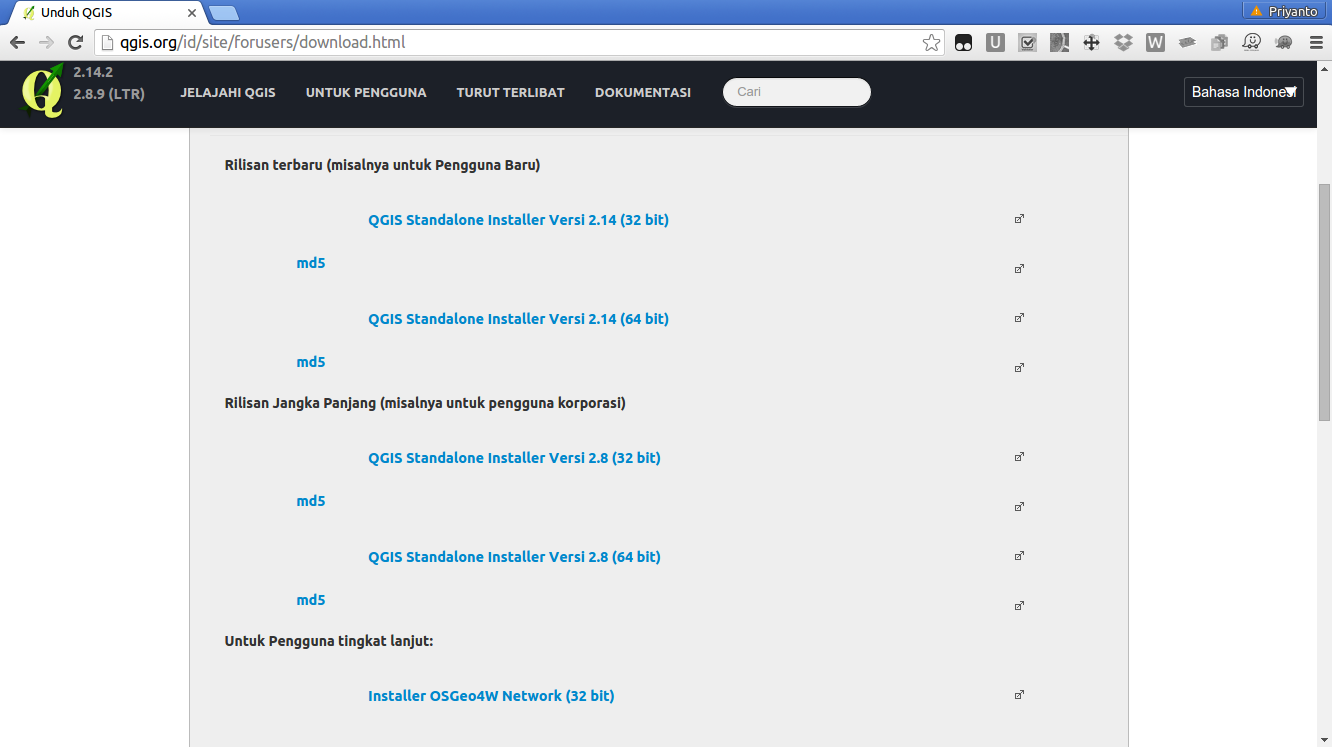
\includegraphics[width=1\textwidth]{./resources/002-pilihan-versi}
  \caption{Pilihan Versi QGIS}
  \label{fig:qgisversion}
\end{figure}

\item Apabila QGIS telah berhasil diunduh, cari \textit{file} instalasi pada direktori yang telah anda tentukan sebelumnya.

\item Klik dua kali pada \textit{file} instalasi tersebut untuk memulai penginstalan QGIS.

\end{enumerate}

\item Instalasi QGIS di lingkungan Sistem Operasi Linux (Debian/Ubuntu)

\end{enumerate}
\chapter{PENGENALAN ANTARMUKA DAN MENAMBAHKAN DATA SIG PADA APLIKASI QGIS}

Pada Bab ini kita akan mengenal bagian-bagian dasar yang biasa digunakan untuk membuat peta menggunakan QGIS 2.14, menambahkan data, dan mengeksplor data menggunakan \textit{tools-tools} yang tersedia.

\begin{enumerate}[A.]

\item \textbf{Pengenalan Antarmuka QGIS 2.14 Essen}

Bagian-bagian dari antarmuka QGIS ini seperti terlihat pada gambar \ref{fig:bagianui}.

\begin{figure}
  \centering
  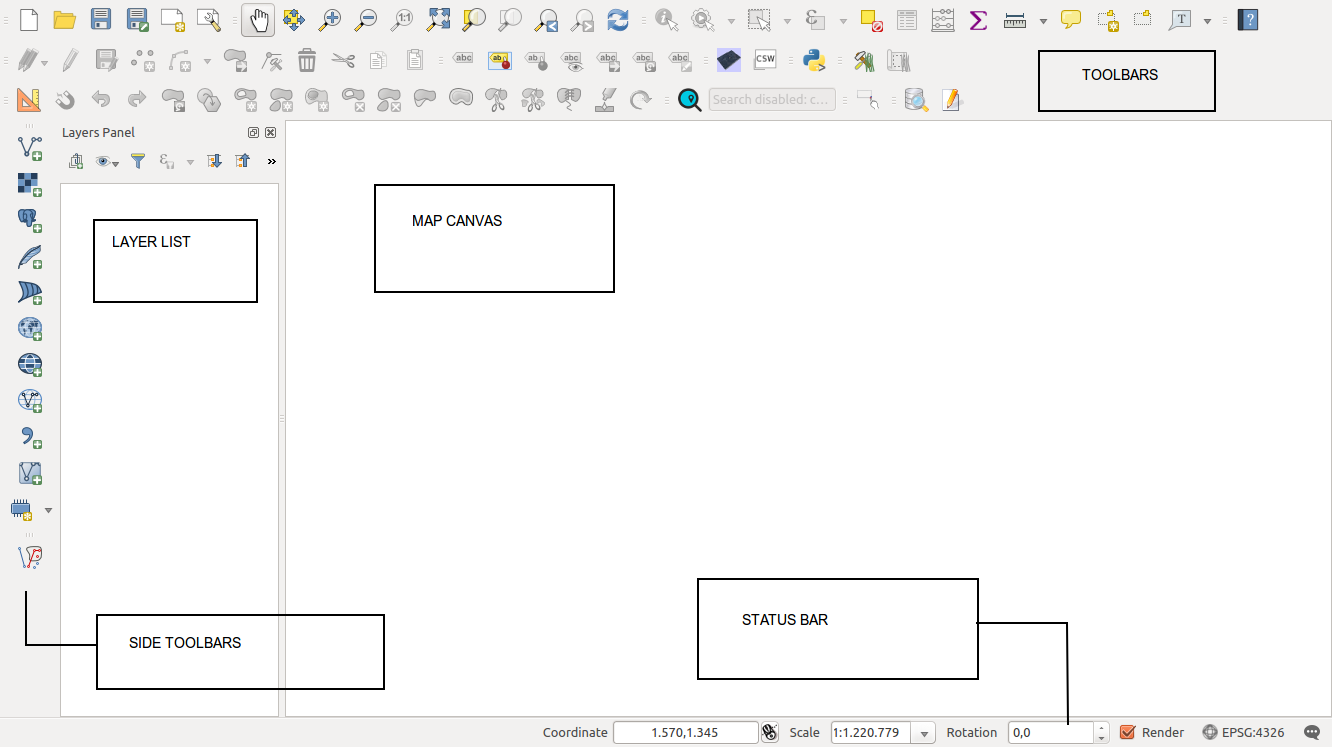
\includegraphics[width=1\textwidth]{./resources/004-bagian-qgis}
  \caption{Bagian Antarmuka QGIS}
  \label{fig:bagianui}
\end{figure}

\begin{itemize}

\item \textbf{Map Canvas}

Merupakan tempat menampilkan proyek / peta yang sedang dijalankan.

\item \textbf{Layer List}

Memuat daftar \textit{layer-layer} yang digunakan dalam proyek. Urutan \textit{layer} yang ditampilkan pada \textit{map canvas} berdasarkan urutan dari atas ke bawah pada \textit{layer list}-nya.

\item \textbf{Menu}

Bagian \textit{menu} ini tidak terlihat di gambar karena konfigurasi tampilan \textit{menu} menempel pada \textit{menu bar desktop}. \textit{Menu} ini berisi sekumpulan perintah teks untuk melakukan tugas-tugas tertentu.

\item \textbf{Toolbar dan Side Tooldbar}

Bagian ini berisi sekumpulan perintah berbasis tombol / ikon untuk melakukan tugas-tugas tertentu. \textit{Tools} dikelompokan dalam grup-grup \textit{toolbar} seperti \textit{File Toolbar}, \textit{Digitizing Toolbar}, \textit{Managed Layers Toolbar}, dan lainnya.

\item \textbf{Status Bar}

\textit{Status bar} memuat koordinat berdasarkan lokasi kursor / pointer, skala, dan sistem koordinat proyek pada \textit{map canvas}.

\end{itemize}

\item \textbf{Menambahkan Data}

Dalam QGIS dan aplikasi GIS pada umumnya, data vektor dalam format \textit{shapefile} dan data \textit{raster} yang akan ditambahkan untuk membuat sebuah \textit{project} (\texttt{*.qgis}) yang telah dibuat, melainkan hanya menyimpan \textit{style} dari data tersebut. Data tetap berada pada \textit{direktori} tempat menyimpan data, oleh karena itu satu \textit{dataset} dapat digunakan untuk berbagai \textit{project}. Berikut langkah-langkah yang dilakukan untuk menambahkan data sebagai \textit{layer} dalam QGIS.

\begin{enumerate}[1.]
  \item Klik \textit{tool} \texttt{Add Vector Layer} yang terlihat seperti pada gambar \ref{fig:addvectorlayer}.
  
\begin{figure}[H]
  \centering
  
\includegraphics[scale=1]{./resources/005-ikon-add-vektor-layer}
  \caption{Ikon \textit{Add Vector Layer}}
  \label{fig:addvectorlayer}
\end{figure}

  \item Sebuah kotak dialog tempat untuk memilih \textit{file} yang akan ditambahkan ke dalam proyek QGIS akan muncul seperti pada gambar \ref{fig:addvectorlayerwindow}
  
\begin{figure}[H]
  \centering
  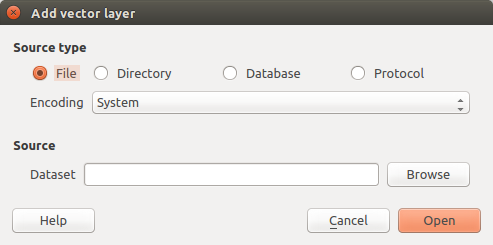
\includegraphics[scale=0.8]{./resources/006-add-vector-layer-window}
  \caption{Jendela \textit{Add Vector Layer}}
  \label{fig:addvectorlayerwindow}
\end{figure}

\end{enumerate}

\item \textbf{Mengeksplor Data}

\end{enumerate} 
\include{07.digitasi-on-screen} 
\include{08.query} 

\backmatter%%%%%%%%%%%%%%%%%%%%%%%%%%%%%%%%%%%%%%%%%%%%%%%%%%%%%%%
\printindex

%%%%%%%%%%%%%%%%%%%%%%%%%%%%%%%%%%%%%%%%%%%%%%%%%%%%%%%%%%%%%%%%%%%%%%

\end{document}





